\documentclass[11pt,a4paper]{ctexart}
\usepackage[margin=2.4cm]{geometry}
\usepackage{amsmath,amssymb}
\usepackage{graphicx}
\usepackage{booktabs}
\usepackage{array}
\usepackage{float}
\usepackage{listings}
\usepackage{xcolor}
\usepackage{caption}
\usepackage[hidelinks]{hyperref}

\pagestyle{plain}
\setcounter{secnumdepth}{-1}
\linespread{1.30}
\captionsetup{font=small}
\setlength{\parskip}{0.35em}

\lstset{
  basicstyle=\ttfamily\footnotesize,
  breaklines=true,
  columns=fullflexible,
  keepspaces=true,
  showstringspaces=false,
  frame=none,
  numbers=none,
  xleftmargin=0.6em,
  aboveskip=0.5em,
  belowskip=0.8em,
}

\title{2026 运筹与优化团队招新考核题 作答}
\author{姓名：兰囿颉}
\date{}

\begin{document}
\maketitle

\section{一、问答题（必做）}

查阅资料，了解“美国大学生数学建模竞赛（MCM/ICM，美赛）”与“全国大学生数学建模竞赛（高教社杯，国赛）”的相关信息，结果如下。

\subsection{（1）2026 年两类比赛的起止时间}
\begin{itemize}
  \item 美赛（MCM/ICM）：北京时间 2026 年 1 月 30 日 06:00 至 2026 年 2 月 3 日 09:00。
  \item 国赛（高教社杯）：2026 年 9 月 10 日（周四）18:00 至 9 月 13 日（周日）20:00。
\end{itemize}

\subsection{（2）报名方式、论文提交方式及注意事项}
\begin{itemize}
  \item 美赛：通过 COMAP 官网报名，每队需缴纳约 100 美元报名费，每队最多 3 人；比赛结束后按官方要求在线提交论文 PDF，并注意以美国东部时间为准的报名与提交截止时间。
  \item 国赛：一般由学校统一组织、经赛区组委会报名，部分学校先进行校内选拔；论文通过全国大学生数学建模竞赛管理系统提交，并按要求附承诺书、论文正文与源程序等。
  \item 共同注意事项：不得跨校组队；论文须独立完成；严格遵循题目给定的格式、页数、命名与提交时间；遵守学术诚信，杜绝抄袭与违规使用他人成果。
\end{itemize}

\subsection{（3）组队人数与任务分工}
\begin{itemize}
  \item 一般 3 人一队。
  \item 常见分工为：建模手负责把实际问题抽象为数学模型；编程手负责用 MATLAB、Python 等求解、仿真与可视化；写作手负责论文写作、排版与图表整理。实际比赛中三人通常交叉协作。
\end{itemize}

\subsection{（4）题型}
\begin{itemize}
  \item 美赛 MCM：A 连续型、B 离散型、C 数据洞察；ICM：D 运筹学与网络科学、E 环境科学、F 政策。
  \item 国赛本科组通常为 A、B、C 三题（个别年份或赛区另有 D、E 等）：A 偏物理、工程与微分方程，B 偏优化与规划，C 偏数据、统计与评价。
\end{itemize}

\subsection{（5）各题型常用算法知识}
\begin{itemize}
  \item 连续与物理类：常微分方程数值解（欧拉法、龙格-库塔法）、偏微分方程（有限差分、有限元）、插值与拟合、数值积分、最优化（梯度下降、牛顿法、拟牛顿法）、蒙特卡洛模拟。
  \item 优化与规划类：线性规划（单纯形法）、整数规划与 0-1 规划（分支定界、割平面）、非线性规划（拉格朗日乘子法、KKT 条件）、动态规划、图论与网络流（Dijkstra、Floyd、最小生成树、最大流与最小费用流）、智能优化（遗传算法、粒子群、模拟退火、蚁群算法、禁忌搜索）、排队论、多目标优化与综合评价（TOPSIS、层次分析、熵权法）。
  \item 数据与统计类：回归分析（线性、多元、非线性）、分类（逻辑回归、决策树、随机森林、支持向量机、神经网络）、聚类（K-means、层次聚类、DBSCAN）、主成分分析、因子分析、时间序列（ARIMA、指数平滑）、灰色预测 GM(1,1)、模糊综合评价等。
\end{itemize}

\section{二、基础题（必做）：18 米线材切割建模}

某工厂只能购买统一规格 18 米的铝合金线材，需要切割出下表所示长度与数量的线材，要求至少购买多少根 18 米线材、使浪费最少，并给出切割方案的建模。

\begin{table}[H]
\centering
\begin{tabular}{ccc}
\toprule
编号 & 长度（米） & 数量（根） \\
\midrule
1 & 6.20 & 90 \\
2 & 3.60 & 120 \\
3 & 2.80 & 136 \\
4 & 1.85 & 310 \\
5 & 0.75 & 215 \\
6 & 0.55 & 320 \\
\bottomrule
\end{tabular}
\end{table}

\subsection{2.1 建模思路}
先把所有“一根 18 米原料能切出的组合”枚举成有限个切割模式，再决定每种模式使用多少根原料，从而把连续的切割问题转化为整数规划问题。

\subsection{2.2 决策变量}
设第 $i$ 种线材的长度为 $l_i$、需求量为 $N_i$（$i=1,2,\dots,6$）。对第 $k$ 种切割模式，用 $a_{ik}$ 表示该模式切出第 $i$ 种长度线材的根数，$x_k$ 表示使用第 $k$ 种模式的 18 米原料根数。

\subsection{2.3 目标函数}
总需求长度固定，原料根数越少、总浪费越少，因此目标等价于最小化原料总根数：
\[
\min\ Z=\sum_{k} x_k
\]

\subsection{2.4 约束条件}
模式可行性（在枚举模式时保证）与需求满足约束分别为：
\[
\sum_{i} l_i\,a_{ik}\le 18
\]
\[
\sum_{k} a_{ik}\,x_k\ge N_i,\qquad i=1,2,\dots,6
\]
\[
x_k\ge 0,\qquad x_k\in\mathbb{Z}
\]

\subsection{2.5 下界检验}
总需求长度 $=2281.55$ 米，故原料根数下界为 $\lceil 2281.55/18\rceil=127$ 根。用整数规划求解，127 根可构造出满足全部需求的切割方案（购买总长 2286 米，浪费约 4.45 米），说明 127 根为最优。

\section{三、计算题 A：8 米与 12 米两种原料的线材下料}

可购买 8 米、12 米两种规格的铝合金线材，需切割的长度与数量同基础题。要求设计计算方案，求出至少购买多少根 8 米与 12 米线材使浪费较少，并给出切割方案与线材利用率。

\subsection{3.1 求解方法}
分别枚举 8 米、12 米原料的所有可行切割模式；以每种模式的使用根数为决策变量建立整数规划，目标为最小化购买总长度（需求总长固定，等价于最小化浪费），约束为各长度产出不少于需求。

\subsection{3.2 计算结果}
\begin{table}[H]
\centering
\begin{tabular}{cc}
\toprule
项目 & 结果 \\
\midrule
8 米原料 & 2 根 \\
12 米原料 & 189 根 \\
原料合计 & 191 根 \\
购买总长度 & 2284.00 米 \\
需求总长度 & 2281.55 米 \\
总浪费 & 2.45 米 \\
线材利用率 & 99.8927\% \\
\bottomrule
\end{tabular}
\end{table}

\subsection{3.3 切割方案}
\begin{table}[H]
\centering
\begin{tabular}{cccl}
\toprule
原料 & 根数 & 切割组合 & 用料 \\
\midrule
8 米 & 2 & $1.85\times4+0.55\times1$ & 7.95 米 \\
12 米 & 45 & $6.2\times1+1.85\times2+0.75\times2+0.55\times1$ & 11.95 米 \\
12 米 & 36 & $3.6\times2+1.85\times2+0.55\times2$ & 12.00 米 \\
12 米 & 35 & $3.6\times1+2.8\times3$ & 12.00 米 \\
12 米 & 31 & $6.2\times1+2.8\times1+0.75\times4$ & 12.00 米 \\
12 米 & 28 & $1.85\times5+0.55\times5$ & 12.00 米 \\
12 米 & 13 & $6.2\times1+3.6\times1+0.55\times4$ & 12.00 米 \\
12 米 & 1 & $6.2\times1+0.75\times1+0.55\times9$ & 11.90 米 \\
\bottomrule
\end{tabular}
\end{table}

上述组合恰好切出 $6.2\times90$、$3.6\times120$、$2.8\times136$、$1.85\times310$、$0.75\times215$、$0.55\times320$。总需求 2281.55 米，最大原料 12 米，故根数下界为 $\lceil 2281.55/12\rceil=191$ 根；本方案恰为 191 根，为最优。

\section{四、计算题 B：生鲜冷链配送车辆路径优化}

某生鲜电商平台设有一座中央配送仓库，负责向市区 31 个社区配送站配送生鲜农产品。现有 25 辆冷链配送车，每辆最大载重 50 件标准周转箱；要求使用最少车辆数、规划各车最佳行驶路线，使总配送距离最短，并给出算法实现过程与最优配送方案。

\subsection{4.1 数据说明}
仓库为编号 1，坐标 $(82,76)$，需求量 0；编号 2 至 32 为 31 个配送站。该组数据即经典 CVRP 测试算例 A-n32-k5，本题将单车容量由 100 改为 50。总需求量为 413 件，故车辆数下界为 $\lceil 413/50\rceil=9$ 辆。

\subsection{4.2 求解算法}
\begin{itemize}
  \item 回溯装箱（Bin Packing）：按需求量从大到小排序后回溯装填，确定最少车辆数（9 辆，达到下界）。
  \item 最近邻算法（Nearest Neighbor）：为每辆车的客户组构造初始行驶路线。
  \item 2-opt 局部搜索：对单条路线反复交换边的连接方式以缩短里程。
  \item 邻域搜索：用客户移动与两车客户交换两种邻域操作，在保持车辆数不变的前提下缩短总距离。
  \item 迭代局部搜索（ILS）：在局部搜索之间加入随机扰动并多次重启动，跳出局部最优。
\end{itemize}

\subsection{4.3 计算结果}
最少车辆数为 9 辆，达到理论下界；总配送距离约 1302.09 km。各车路线如下。

\begin{table}[H]
\centering
\begin{tabular}{cccc}
\toprule
车辆 & 载货（件） & 里程（km） & 配送路线 \\
\midrule
1 & 45 & 152.24 & $1\to22\to32\to20\to1$ \\
2 & 44 & 196.37 & $1\to23\to10\to16\to30\to1$ \\
3 & 44 & 59.26 & $1\to28\to25\to1$ \\
4 & 49 & 170.56 & $1\to27\to14\to18\to7\to1$ \\
5 & 40 & 72.02 & $1\to13\to2\to1$ \\
6 & 47 & 174.54 & $1\to11\to26\to6\to21\to1$ \\
7 & 46 & 209.15 & $1\to5\to12\to9\to19\to15\to1$ \\
8 & 50 & 192.48 & $1\to4\to3\to24\to29\to1$ \\
9 & 48 & 75.47 & $1\to31\to17\to8\to1$ \\
\bottomrule
\end{tabular}
\end{table}

\begin{figure}[H]
\centering
\IfFileExists{B_路线图.png}{%
  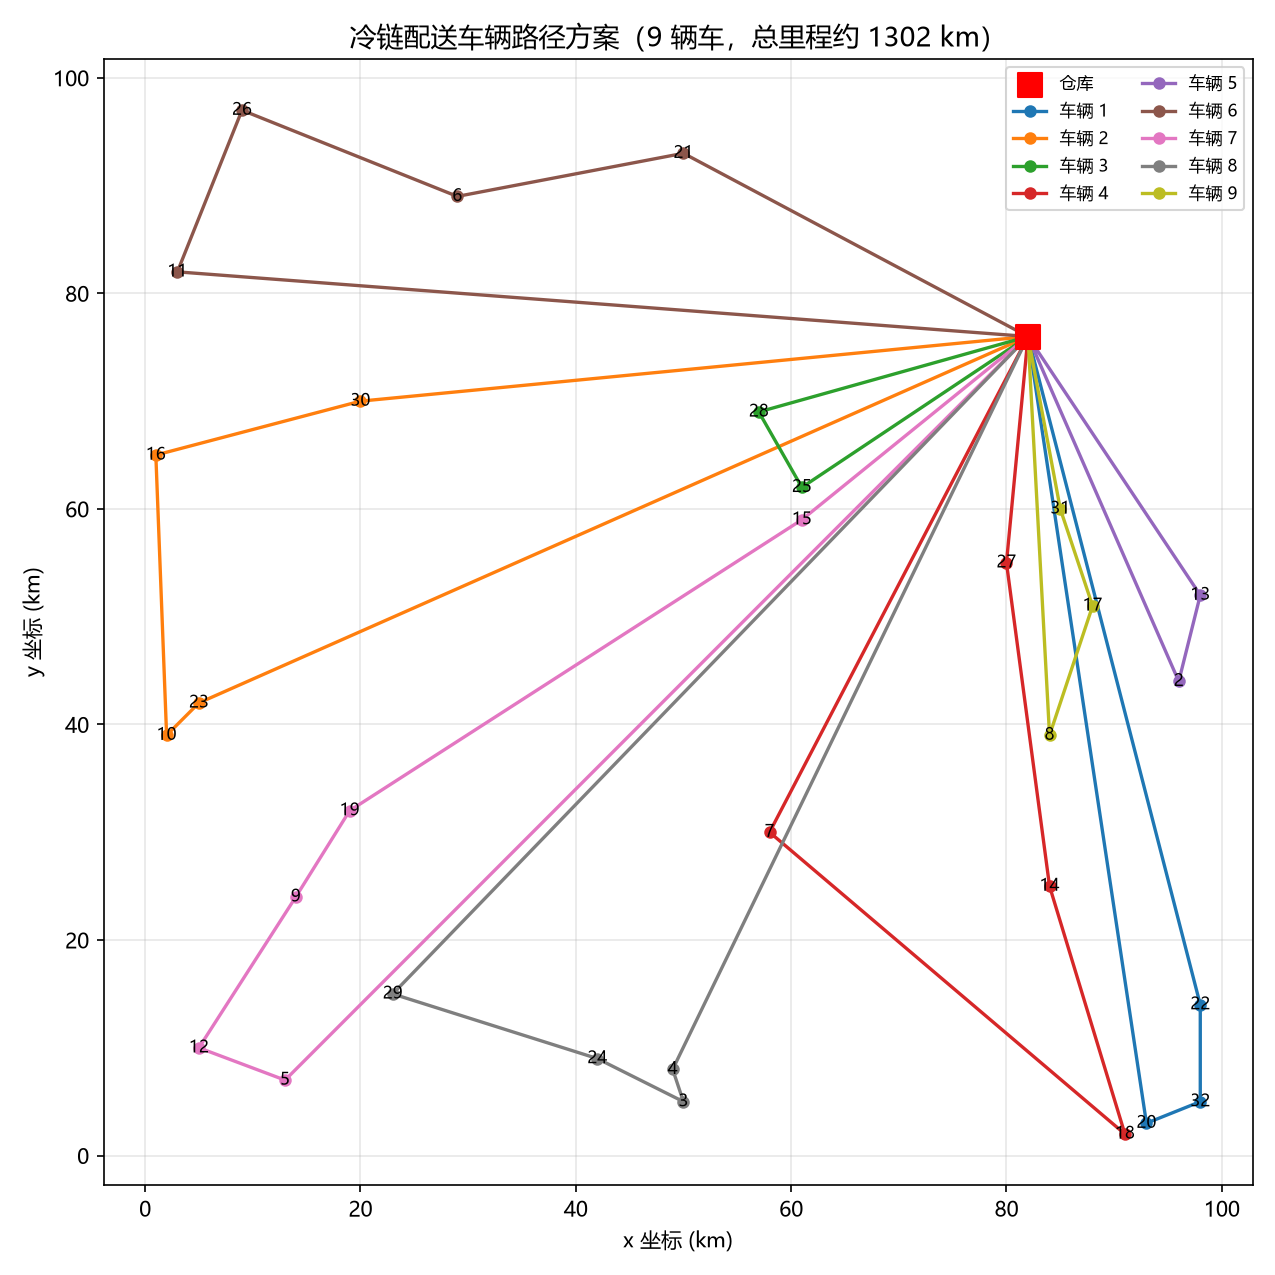
\includegraphics[width=0.86\textwidth]{B_路线图.png}%
}{%
  \fbox{\parbox[c][4.5cm][c]{0.8\textwidth}{\centering 未找到路线图文件 B\_路线图.png；请将图片与本 .tex 文件放在同一目录后重新编译。}}%
}
\caption{冷链配送车辆路径方案（9 辆车，总里程约 1302 km）}
\end{figure}

\clearpage
\section{附录 A  计算题 A 代码（A\_下料.py）}
\begin{lstlisting}
# -*- coding: utf-8 -*-
"""
计算题 A：两种原料（8 米、12 米）铝合金线材下料优化

需求（与题目表格一致）：
    长度  6.20  3.60  2.80  1.85  0.75  0.55（米）
    数量    90   120   136   310   215   320（根）

方法：枚举 8 米、12 米的全部可行“切割模式”，
用整数规划（PuLP + CBC）最小化购买总长度（等价于最小化浪费），
并输出各模式用量、总共需要的 8m/12m 根数、切割方案与线材利用率。
"""

import pulp

# 需求
lengths = [6.20, 3.60, 2.80, 1.85, 0.75, 0.55]
demands = [90, 120, 136, 310, 215, 320]

# 换算成毫米，避免浮点误差
mm = [int(round(l * 1000)) for l in lengths]

# 原料：名称 -> 长度（毫米）
stock_specs = {"8m": 8000, "12m": 12000}


def enumerate_patterns(stock_mm):
    """枚举单根原料上所有可行的切割模式。

    模式用元组 (a1, a2, ..., a6) 表示，ai 为该模式切出第 i 种长度的根数。
    """
    n = len(mm)
    out = []

    def dfs(i, rem, vec):
        if i == n:
            out.append(tuple(vec))
            return
        max_k = min(stock_mm // mm[i], rem // mm[i])
        for k in range(max_k + 1):
            dfs(i + 1, rem - k * mm[i], vec + [k])

    dfs(0, stock_mm, [])
    return out


def main():
    pattern_sets = {name: enumerate_patterns(smm) for name, smm in stock_specs.items()}

    prob = pulp.LpProblem("cutting_stock_A", pulp.LpMinimize)

    # 决策变量：x[name][j] = 第 name 种原料按第 j 个模式切割的根数
    x = {
        name: [
            pulp.LpVariable(f"x_{name}_{j}", lowBound=0, cat=pulp.LpInteger)
            for j in range(len(ps))
        ]
        for name, ps in pattern_sets.items()
    }

    # 目标：最小化购买总长度（毫米）；总需求长度固定，等价于最小化浪费
    prob += pulp.lpSum(
        stock_specs[name] * x[name][j]
        for name in pattern_sets
        for j in range(len(pattern_sets[name]))
    )

    # 约束：每种长度的产出根数不少于需求量
    for i in range(len(mm)):
        prob += (
            pulp.lpSum(
                pattern_sets[name][j][i] * x[name][j]
                for name in pattern_sets
                for j in range(len(pattern_sets[name]))
            )
            >= demands[i],
            f"demand_{i}",
        )

    prob.solve(pulp.PULP_CBC_CMD(msg=0))
    assert pulp.LpStatus[prob.status] == "Optimal", f"未找到最优解: {pulp.LpStatus[prob.status]}"

    used = {name: {} for name in pattern_sets}
    for name in pattern_sets:
        for j, ps in enumerate(pattern_sets[name]):
            v = int(round(x[name][j].value()))
            if v > 0:
                used[name][ps] = v

    n8 = sum(used["8m"].values())
    n12 = sum(used["12m"].values())
    purchased_mm = stock_specs["8m"] * n8 + stock_specs["12m"] * n12
    total_demand_mm = sum(mm[i] * demands[i] for i in range(len(mm)))
    waste_mm = purchased_mm - total_demand_mm

    print("=" * 70)
    print("计算题 A 求解结果")
    print("=" * 70)
    print(f"需要 8 米原料：{n8} 根")
    print(f"需要 12 米原料：{n12} 根")
    print(f"购买总长度：{purchased_mm / 1000:.2f} 米")
    print(f"需求总长度：{total_demand_mm / 1000:.2f} 米")
    print(f"总浪费：{waste_mm / 1000:.2f} 米")
    print(f"线材利用率：{total_demand_mm / purchased_mm * 100:.4f}%")
    print()

    print("切割方案（模式 -> 使用根数）：")
    for name in ["8m", "12m"]:
        print(f"\n[{name} 原料]")
        for ps, cnt in sorted(used[name].items(), key=lambda kv: -kv[1]):
            pieces = [f"{lengths[i]}×{ps[i]}" for i in range(len(mm)) if ps[i] > 0]
            used_len = sum(mm[i] * ps[i] for i in range(len(mm)))
            print(f"  切 {cnt:3d} 根 | {' + '.join(pieces):40s} 用料 {used_len/1000:.2f}m")


if __name__ == "__main__":
    main()
\end{lstlisting}

\clearpage
\section{附录 B  计算题 B 代码（B\_配送.py）}
\begin{lstlisting}
# -*- coding: utf-8 -*-
"""
计算题 B：生鲜冷链配送车辆路径问题（CVRP）

数据：1 个仓库 + 31 个配送站（文档编号 1 为仓库，2~32 为配送站），
单车容量 50 件，可用车辆上限 25 辆。距离采用欧氏距离（单位：km）。

求解思路：
1. 先用“装箱（bin packing）”确定最少车辆数（由总需求 413 件 / 容量 50 得下界 9 辆，
   并用回溯法验证 9 辆可行）；
2. 对每辆车的客户组分别用“最近邻 + 2-opt”构造行驶路线；
3. 用“迭代局部搜索（ILS）”：在保持 9 辆车不变的前提下，通过客户在车辆间
   移动 / 交换、随机扰动与重启动，持续缩短总配送距离。
"""

import math
import random

# 仓库（文档编号 1）
DEPOT = (1, 82.0, 76.0, 0)

# 配送站：文档编号 2~32，坐标为 (x, y)，需求量为件/天
CUSTOMERS = [
    (2, 96, 44, 19), (3, 50, 5, 21), (4, 49, 8, 6), (5, 13, 7, 19),
    (6, 29, 89, 7), (7, 58, 30, 12), (8, 84, 39, 16), (9, 14, 24, 6),
    (10, 2, 39, 16), (11, 3, 82, 8), (12, 5, 10, 14), (13, 98, 52, 21),
    (14, 84, 25, 16), (15, 61, 59, 3), (16, 1, 65, 22), (17, 88, 51, 18),
    (18, 91, 2, 19), (19, 19, 32, 4), (20, 93, 3, 24), (21, 50, 93, 8),
    (22, 98, 14, 12), (23, 5, 42, 4), (24, 42, 9, 8), (25, 61, 62, 24),
    (26, 9, 97, 24), (27, 80, 55, 2), (28, 57, 69, 20), (29, 23, 15, 15),
    (30, 20, 70, 2), (31, 85, 60, 14), (32, 98, 5, 9),
]

CAPACITY = 50
MAX_VEHICLES = 25


def dist(a, b):
    return math.hypot(a[1] - b[1], a[2] - b[2])


def route_length(route, nodes):
    return sum(dist(nodes[route[k]], nodes[route[k + 1]]) for k in range(len(route) - 1))


def route_demand(route, nodes):
    return sum(nodes[i][3] for i in route if i != 0)


def two_opt(route, nodes):
    """对单条路线做 2-opt 局部优化。"""
    improved = True
    while improved:
        improved = False
        best = route_length(route, nodes)
        for a in range(1, len(route) - 2):
            for b in range(a + 1, len(route) - 1):
                new_route = route[:a] + list(reversed(route[a:b + 1])) + route[b + 1:]
                new_len = route_length(new_route, nodes)
                if new_len < best - 1e-9:
                    route, best = new_route, new_len
                    improved = True
                    break
            if improved:
                break
    return route


def pack_into_k(demands, k, capacity):
    """回溯装箱：把 31 个需求装入 k 个容量为 capacity 的箱子。"""
    items = sorted(range(len(demands)), key=lambda i: -demands[i])
    bins = [[] for _ in range(k)]
    loads = [0] * k

    def bt(idx):
        if idx == len(items):
            return True
        it = items[idx]
        d = demands[it]
        for b in range(k):
            if loads[b] + d <= capacity:
                bins[b].append(it)
                loads[b] += d
                if bt(idx + 1):
                    return True
                bins[b].pop()
                loads[b] -= d
        return False

    return bins if bt(0) else None


def route_group(member_ids, nodes):
    """对一组客户（节点编号集合）用最近邻 + 2-opt 构造路线。"""
    unvisited = set(member_ids)
    route = [0]
    cur = 0
    while unvisited:
        nxt = min(unvisited, key=lambda k: dist(nodes[cur], nodes[k]))
        route.append(nxt)
        unvisited.remove(nxt)
        cur = nxt
    route.append(0)
    return two_opt(route, nodes)


def local_search(routes, nodes, capacity):
    """在保持车辆数不变的前提下，用客户移动/交换缩短总里程。"""
    improved = True
    while improved:
        improved = False
        best = None

        # 移动：把 a 路线里的一个客户插入到 b 路线
        for a in range(len(routes)):
            for i in range(1, len(routes[a]) - 1):
                node = routes[a][i]
                if len(routes[a]) <= 3:  # 路线里只有一个客户时不移动，避免车辆数增加
                    continue
                for b in range(len(routes)):
                    if a == b:
                        continue
                    if route_demand(routes[b], nodes) + nodes[node][3] > capacity:
                        continue
                    for pos in range(1, len(routes[b])):
                        new_a = routes[a][:i] + routes[a][i + 1:]
                        new_b = routes[b][:pos] + [node] + routes[b][pos:]
                        delta = (route_length(new_a, nodes) + route_length(new_b, nodes)) - (
                            route_length(routes[a], nodes) + route_length(routes[b], nodes)
                        )
                        if delta < -1e-9 and (best is None or delta < best[0]):
                            best = (delta, "move", a, b, i, pos)

        # 交换：a、b 两条路线各取一个客户互换
        for a in range(len(routes)):
            for b in range(a + 1, len(routes)):
                for i in range(1, len(routes[a]) - 1):
                    for j in range(1, len(routes[b]) - 1):
                        na, nb = routes[a][i], routes[b][j]
                        if route_demand(routes[a], nodes) - nodes[na][3] + nodes[nb][3] > capacity:
                            continue
                        if route_demand(routes[b], nodes) - nodes[nb][3] + nodes[na][3] > capacity:
                            continue
                        new_a = routes[a][:i] + [nb] + routes[a][i + 1:]
                        new_b = routes[b][:j] + [na] + routes[b][j + 1:]
                        delta = (route_length(new_a, nodes) + route_length(new_b, nodes)) - (
                            route_length(routes[a], nodes) + route_length(routes[b], nodes)
                        )
                        if delta < -1e-9 and (best is None or delta < best[0]):
                            best = (delta, "swap", a, b, i, j)

        if best is None:
            break
        delta, kind, a, b, i, j = best
        if kind == "move":
            node = routes[a][i]
            routes[a] = routes[a][:i] + routes[a][i + 1:]
            routes[b] = routes[b][:j] + [node] + routes[b][j:]
        else:
            na, nb = routes[a][i], routes[b][j]
            routes[a] = routes[a][:i] + [nb] + routes[a][i + 1:]
            routes[b] = routes[b][:j] + [na] + routes[b][j + 1:]
        routes[a] = two_opt(routes[a], nodes)
        routes[b] = two_opt(routes[b], nodes)
        improved = True

    return routes


def iterated_local_search(groups0, nodes, capacity, iters=600, seed=7):
    """迭代局部搜索：在固定车辆数下尽量缩短总里程。"""
    demands = [nodes[i][3] for i in range(1, len(nodes))]
    rng = random.Random(seed)
    groups = [list(g) for g in groups0]
    best = None

    def make(g):
        return [route_group([i + 1 for i in gg], nodes) for gg in g if gg]

    def total(routes):
        return sum(route_length(r, nodes) for r in routes)

    for _ in range(iters):
        routes = local_search(make(groups), nodes, capacity)
        d = total(routes)
        if best is None or d < best[0]:
            best = (d, routes, [list(g) for g in groups])

        gs = [list(g) for g in (best[2] if rng.random() < 0.4 else groups)]
        for _ in range(4):
            a, b = rng.sample(range(len(gs)), 2)
            if not gs[a] or not gs[b]:
                continue
            x = rng.choice(gs[a])
            y = rng.choice(gs[b])
            da = sum(demands[i] for i in gs[a])
            db = sum(demands[i] for i in gs[b])
            if da - demands[x] + demands[y] <= capacity and db - demands[y] + demands[x] <= capacity:
                gs[a].remove(x)
                gs[a].append(y)
                gs[b].remove(y)
                gs[b].append(x)
        groups = gs

    return best[1]


def plot_routes(routes, nodes, out="B_路线图.png"):
    try:
        import matplotlib
        matplotlib.use("Agg")
        import matplotlib.pyplot as plt
        from matplotlib import font_manager

        # 尽量使用中文字体，避免中文显示成方框
        for fname in ["Microsoft YaHei", "SimHei", "SimSun"]:
            try:
                font_manager.findfont(fname, fallback_to_default=False)
                plt.rcParams["font.sans-serif"] = [fname]
                break
            except Exception:
                continue
        plt.rcParams["axes.unicode_minus"] = False

        total = sum(route_length(r, nodes) for r in routes)
        fig, ax = plt.subplots(figsize=(8.5, 8.5))
        colors = plt.cm.tab10.colors
        ax.scatter([DEPOT[1]], [DEPOT[2]], c="red", marker="s", s=130, zorder=5, label="仓库")
        for k, r in enumerate(routes):
            xs = [nodes[i][1] for i in r]
            ys = [nodes[i][2] for i in r]
            ax.plot(xs, ys, marker="o", markersize=5, linewidth=1.6,
                    color=colors[k % 10], label=f"车辆 {k + 1}")
        for c in CUSTOMERS:
            ax.annotate(str(c[0]), (c[1], c[2]), fontsize=8, ha="center", va="center")
        ax.set_title(f"冷链配送车辆路径方案（{len(routes)} 辆车，总里程约 {total:.0f} km）", fontsize=13)
        ax.set_xlabel("x 坐标 (km)")
        ax.set_ylabel("y 坐标 (km)")
        ax.legend(fontsize=8, ncol=2, loc="best")
        ax.grid(True, alpha=0.3)
        fig.tight_layout()
        fig.savefig(out, dpi=150)
        plt.close(fig)
    except Exception as e:  # 绘图失败不影响主流程
        print(f"(绘图跳过：{e})")


def main():
    nodes = [DEPOT] + CUSTOMERS
    demands = [c[3] for c in CUSTOMERS]
    total_demand = sum(demands)
    lower = math.ceil(total_demand / CAPACITY)

    # 1. 确定最少车辆数
    groups = None
    for k in range(lower, MAX_VEHICLES + 1):
        g = pack_into_k(demands, k, CAPACITY)
        if g is not None:
            groups = g
            break

    # 2. 用迭代局部搜索在最少车辆数下优化路线与总里程
    routes = iterated_local_search(groups, nodes, CAPACITY)

    total_distance = sum(route_length(r, nodes) for r in routes)

    print("=" * 72)
    print("计算题 B 求解结果（装箱定车辆数 + 最近邻/2-opt + 迭代局部搜索）")
    print("=" * 72)
    print(f"配送站总数：{len(CUSTOMERS)}，总需求量：{total_demand} 件")
    print(f"车辆容量：{CAPACITY} 件，车辆数下界：{lower} 辆")
    print(f"本方案使用车辆数：{len(routes)} 辆（上限 {MAX_VEHICLES} 辆）")
    print(f"总配送距离：{total_distance:.2f} km")
    print()
    for idx, r in enumerate(routes, 1):
        demand = route_demand(r, nodes)
        length = route_length(r, nodes)
        seq = " -> ".join(str(nodes[i][0]) for i in r)
        print(f"车辆 {idx:2d} | 载货 {demand:2d} 件 | 里程 {length:6.2f} km | 路线：{seq}")

    plot_routes(routes, nodes)
    return routes, nodes


if __name__ == "__main__":
    main()
\end{lstlisting}

\end{document}
